\documentclass[12pt]{exam}
\usepackage[utf8]{inputenc}
\usepackage[margin=1in]{geometry}
\usepackage{amsmath,amssymb}
\usepackage{multicol}
\usepackage[english]{babel}
\usepackage{graphicx}
\usepackage{tikz}
\usepackage{float}
\usepackage{etoolbox} % Required for \ifblank
\usepackage{xcolor} % Required for comments or highlighting
\usepackage{tabularx}
\usepackage{setspace} % Required for setting line spacing


\newcommand{\class}{Fundamentals of Thermal Sciences}
\newcommand{\term}{DE-46 MTS}
\newcommand{\examnum}{Midterm Exam Practice Problems}
\newcommand{\examdate}{Mar 4, 2026}
\newcommand{\timelimit}{-- hours}
\newcommand{\classcode}{ME-474}
\newcommand{\timing}{-- hrs}
\newcommand{\maxmarks}{--}
\newcommand{\Instructor}{Usman Asad}

\pagestyle{head}
\firstpageheader{\textbf{CMS ID} \makebox[1.5in]{\hrulefill}}{}{Page \thepage\ of \numpages}
\runningheader{}{Page \thepage\ of \numpages}{}
\runningheadrule


% Top Stuff
\begin{document}
	\begin{tikzpicture}[remember picture,overlay]
		\node[xshift=25 mm,yshift=-30 mm,anchor=north west] at (current page.north west){%
			\includegraphics[width=24mm]{NUST}};
	\end{tikzpicture}

	\begin{tikzpicture}[remember picture,overlay]
		\node[xshift=-25 mm,yshift=-30 mm,anchor=north east] at (current page.north east){%
			\includegraphics[width=24mm]{CEME}};
	\end{tikzpicture}

	\begin{center}
		\textbf{National University of Sciences and Technology}\\
		\textbf{College of E\&ME (Department of Mechatronics)}\\
		\textbf{\examnum (\term)}\\
	\end{center}

	% Exam Details
	\noindent

	\begin{tabular*}{\textwidth}{l @{\extracolsep{\fill}} r @{\extracolsep{6pt}} l}
		\textbf{Subject Code: }\classcode &&\textbf{Subject: }\class \\
		\textbf{Date: }\examdate && \textbf{Timing: }\timing\\
		\textbf{Time Limit: }\timelimit && \textbf{Max Marks: }\maxmarks\\
		\textbf{Instructor: }\Instructor
	\end{tabular*}\\
	\rule[2ex]{\textwidth}{1pt}
	\textbf{Instructions:}\\This document contains \numpages\ pages. These are a collection of previous exam and assignment questions over the years, based on the material already covered in the course\\ \\
	\rule[2ex]{\textwidth}{1pt}

	\begin{questions}

		% True False
		\question[5] Mark box if true.
		\addpoints
		\begin{checkboxes}
			\choice The units of specific heat is kJ/kg [False]
			\choice Density of a fluid is an extensive property [False]
			\choice An Open System is also called a Control Volume [True]
			\choice Heat transfer is equal to Work done in an adiabatic process [False]
			\choice If the pressure and Temperature of water is known, we can determine its specific volume [True]
			
		\end{checkboxes}
		
		
		
		{%
			% changing choice items style locally
			%\renewcommand*\thechoice{\arabic{choice}} 
			%\renewcommand*\choicelabel{\thechoice)}
			%
		
			
		}%
		
		\renewcommand{\baselinestretch}{3}
		\question[10] Fill in the blanks
			\begin{parts}
				\part The gage pressure of tank is 20 psi. The absolute pressure will be \textbf{34.7 psi}
				\part A 4 kW electric heater is kept on in room for 15 mins. The amount of energy transfered to the room is \textbf{3600} kJ
				\part A mercury barometer is used to measure atmospheric pressure. The height of the mercury column will be around \textbf{760 mm / 30 in} The specific weight of mercury is $\lambda=\rho g=0.49\ lb/in^3=133.7\ kN/m^3$ and $1\ atm=14.7\ psi=101.325\ kPa$ 
				\part $45^o\ C$ is equal to \textbf{113} Fahrenheit
				\part The SI unit of thermal conductivity 'k' is W/mK
				\part 150 lbf converted in to SI units is \textbf{667.2 N}
				\part 700 N converted in to kgf is \textbf{71.4 kgf} 
				\part The vacuum pressure of tank is 5 psi. The absolute pressure will be \textbf{9.7 psi}
				\part $273\ K$ is equal to \textbf{32} Fahrenheit
				\part The SI unit of the Stefan Boltzmann constant '$\sigma$' is \textbf{$W/m^2K^4$}
	%			
				
			\end{parts}	

			\question[10] Consider a double-fluid manometer attached to an air pipe shown in figure below. If the specific gravity of one fluid is 13.55, determine the specific gravity and density of the other fluid for the indicated absolute pressure of air. Take the atmospheric pressure to be 100 kPa 
	\begin{center}
		
		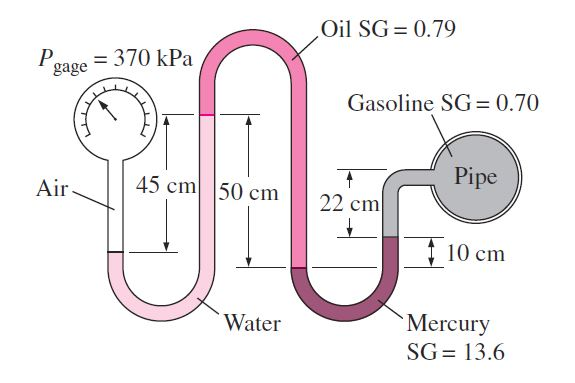
\includegraphics[width=0.4\linewidth]{S1-1} \\
		
	\end{center}
	\textbf{Solution:} \\
	$$P_{atm}+\rho_2gh_2-\rho_1gh_1=P_{air}$$
	$$\to 100000+\rho_2\times9.8\times0.4-13550\times9.8\times0.22=76000$$
	Solving for $\rho_2$, gives us $\rho_2=1330\ kg/m^3$, so $SG_2=1.33$ \\
	Note: This is Problem 1-76 from the Cengel and Boles textbook.

		\question[30] Consider 2 kg of air in a Piston-Cylinder assembly with the following processes in a thermodynamic cycle:
	\begin{itemize}
		\item \textbf{Process $1\to2$:} Adiabatic compression where $P_1V_1^n=P_2V_2^n$, with $n=1.385$ from atmospheric pressure and $V_1=3\ m^3$to a final volume of $V_2=1\ m^3$
		\item \textbf{Process $2\to3$:} Isothermal expansion to back to atmospheric pressure
		\item \textbf{Process $3\to1$:} Isobaric compression 
		
	\end{itemize}
	
	Draw the cycle on a P-V diagram. \textbf{Evaluate} the work done in each process. \textbf{Evaluate} the heat transfer for each process. \textbf{Estimate} the thermodynamic efficiency of the cycle.
	
	Note that for a polytropic process $PV^n=const$:\\
	$$ n=0\to W_{12}=P(V_2-V_1)$$\\
	$$  n=1\to W_{12}=P_1V_1 \ln(\frac{V_2}{V_1})$$ \\
	Otherwise:
	$$  W_{12}=\frac{P_2V_2-P_1V_1}{1-n}$$\\
	Use the following constants for Air\\
	$R=0.287\ kJ/kgK \quad ; \quad c_p=1.033\ kJ/kgK \quad ; \quad c_v=0.7457\ kJ/kgK$ \\
	
	\textbf{Solution:} \\
	Taking atmospheric pressure to be 100 kPa, pressure at 2 is given by: $$P_2=P_1(V_1/V_2)^n=457.8\ kPa$$ 
	Work done for 1 to 2 is:
	$$  W_{12}=\frac{P_2V_2-P_1V_1}{1-n}=-410.2 kJ\\$$
	Process 2 to 3 is isothermal. Volume at 3 is given by:
	$$P_2V_2=P_3V_3\to V_3=(P_2/P_3)V_2=4.58\ m^3$$
	Work done for the isothermal process (n=1) is:
		$$  W_{23}=P_2V_2\ln(\frac{V_3}{V_2})=696.7\ kJ$$\\
	Work done for for process 3 to 1:
	$$W_{31}=P(V_1-V_3)=-157.9\ kJ$$
	Before we calculate heat transfer, we need the temperatures. At point 1:
	$$P_1V_1=mRT_1\to T_1=249.4^o\ C$$
	$$P_2V_2=mRT_2\to T_2=524.5^o\ C$$
	and $T_2=T_3$ because its an isothermal process
	Heat transfer for process 1 to 2 is zero because its an adiabatic process
	Heat transfer for process for process 2 to 3 is equal to the work done, because of the 1st law:
	$$\Delta U_{23}=Q_{23}-W_{23}$$
	For $\Delta U_{23}=0$ because temperature at 2 and 3 are the same, we have $=Q_{23}=W_{23}=696.7\ kJ$. This is $Q_{in}$ \\
	Process 3 to 1 is a constant pressure process, so:
	$$Q_{31}=mc_p(T_1-T_3)=-568.1\ kJ$$
	So $Q_{out}=568.1\ kJ$. Finally efficiency is:
	$$\eta=1-\frac{Q_{out}}{Q_{in}}=0.1845\ or\ 18.45\%$$
	
	The Pv diagram:
	\begin{center}
		
		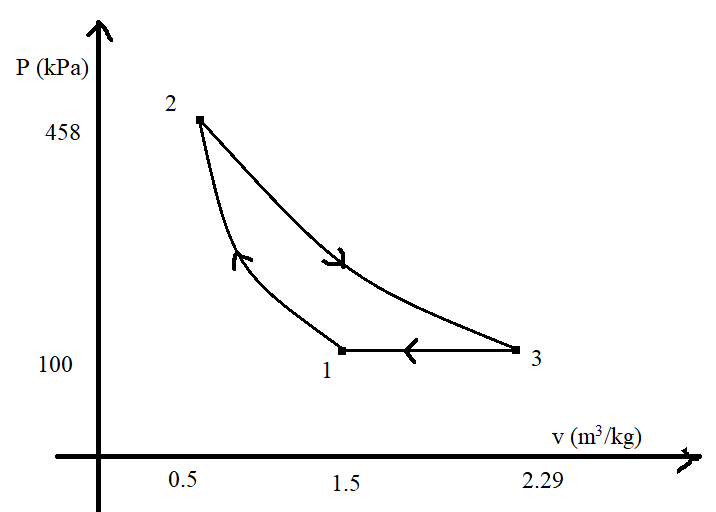
\includegraphics[width=1\linewidth]{S1Q3-PV} \\
		
	\end{center}
	
	Note: PV diagram looks exactly the the same. Just multiply the values of specific volume given the bottom with m=2
		\question[10] Ambient air at a temperature of $25^o$C and a pressure of 100 kPa in a piston cylinder assembly is compressed (in an adiabatic, reversible process) from a volume of 78 $cm^3$ to 8.2 $cm^3$. Estimate the mass of the air. What will be the temperature and pressure of air after compression? How much work will be required for this process? 
		
		\question[10] An average household consumes around 360 kWh of electrical energy per month. Assuming all that energy came from Natural Gas Power plants having an efficiency of around 60\%. In order to judge the environmental impact of an average household, estimate the $CO_2$ emissions due to one household, in kg/year.  Assume that during combustion of natural gas, around 50 kg of $CO_2$ are produced per 1 million kJ of heat released. 				
		\question[10] 
		A gasoline line is connected to a pressure gage through a double-U manometer, as shown in the figure. If the reading of the pressure gage is 370 kPa, determine the gage pressure of the gasoline line.
			
		\begin{center}
			
			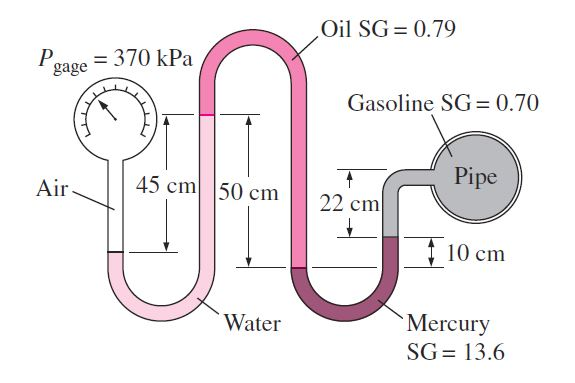
\includegraphics[width=0.6\linewidth]{S1-1} \\

		\end{center}
		
		\textbf{Solution:} \\
		$$P_{petrol}+\rho_{petrol}g(0.22)+\rho_{Hg}g(0.1)-\rho_{Oil}g(0.50)+\rho_{H2O}g(0.45)=370,000$$
		$$P_{petrol}=354.6 kPa$$
		
		
		\question[25] Consider air in a Piston-Cylinder assembly with the following processes in a thermodynamic cycle:
		\begin{itemize}
		\item \textbf{Process $1\to2$:} Adiabatic compression where $P_1V_1^k=P_2V_2^k$, with $k=1.35$ from $P_1=100\ kPa$, $V_1=522.7\ cm^3$, $T_1=333 K$ to $V_2=22.7\ cm^3$, $T_2=996.5 K$
		\item \textbf{Process $2\to3$:} Constant Pressure expansion to $V_3=79.7\ cm^3$
		\item \textbf{Process $3\to4$:} Adiabatic expansion where $P_3V_3^k=P_4V_4^k$, with $k=1.35$  to $V_4=522.7\ cm^3$
		\item \textbf{Process $4\to1$:} Constant Volume Process
		
		\end{itemize}
		
	Draw the cycle on a P-V diagram. \textbf{Estimate} the mass of air in the cylinder. \textbf{Evaluate} the work done in each process. \textbf{Estimate} the thermodynamic efficiency of the cycle, give by:
	$$\eta=\frac{W_{cycle}}{Q_{23}}$$
	
	\textbf{Solution:} \\
	The mass of the air in the cylinder is given by:
	$$m=\frac{P_1V_1}{RT_1}=\frac{100\times 522.7\times 10^{-6}}{0.287\times333}=0.55\times10^{-3}\ kg$$
	Note that the mass doesn't change. You can use values at any state.\\
	
	Pressure after process $1\to2$ is given by:
	$$P_2=P_1(\frac{V_1}{V_2})^k=100\times(\frac{522.7}{22.7})^{1.35}=6902\ kPa$$
	Work done in Process $1\to2$:
	$$W_{12}=\frac{P_2V_2-P_1V_2}{1-k}=-298\ J$$
	
	Work done in Process $2\to3$:
	$$W_{23}=P_2(V_3-V_2)=	393.4\ J$$
	
	Using the same equations as before, Pressure $P_4=544.9\ kPa$, and Work done in Process $3\to4$: $W_{34}=758\ J$
	
	There is no work done in Process $4\to1$ \\
	Net Work done is the cycle is: $W_{cycle}=W_{12}+W_{23}+W_{34}=853.1\ J$
	
	Heat added for Process $2\to3$ is given by:
	$$Q_{23}=\Delta H=mc_p\Delta T=mc_p(T_3-T_2)$$
	The temperature at 3 is given by (using the Ideal Gas Law):
	$$T_3/V_3=T_2/V_2\to T_3=3500 K$$
	$$\to Q_{23}=2724\ J$$
	Finally, the efficiency is:
	$$\eta=\frac{W_{cycle}}{Q_{23}}=31.32\%$$
	
	The PV diagram of the cycle will essentially look like this:	
	\begin{center}
		
		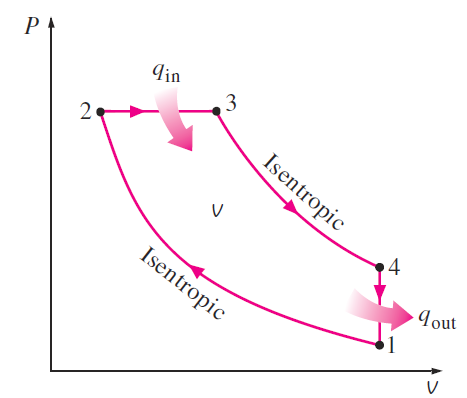
\includegraphics[width=0.6\linewidth]{S1-S} \\
		
	\end{center}	
	
	This cycle is the called the Air-Standard Diesel Cycle. The problem we solved is an approximation for one of the pistons of the Toyota Corolla 2.0D

	
		\question A piston–cylinder device contains helium gas initially at 150 kPa, 20$^{\circ}$C, and 0.5 m3. The helium is now compressed in a polytropic process ($PV^n=$constant) to 400 kPa and 140$^{\circ}$C. Determine the heat loss or gain during this process. \\Answer: 11.2 kJ loss

		\question A 0.5 $m^3$ rigid tank contains refrigerant-134a initially at 200 kPa and 40 percent quality. Heat is transferred now to the refrigerant from a source at 35$^{\circ}$C until the pressure rises to 400 kPa. Determine (a) the entropy change of the refrigerant, (b) the entropy change of the heat source, and (c) the total entropy change for this process. \\Answers: (a) 3.880 kJ/K, (b) 3.439 kJ/K, (c) 0.441 kJ/K

		\question The inner and outer surfaces of a $5m \times 6m$ brick wall of thickness 30 cm and thermal conductivity 0.69 W/m$^{\circ}$C are maintained at temperatures of 20$^{\circ}$C and 5$^{\circ}$C, respectively. Determine the rate of heat transfer through the wall, in W.
		\begin{center}
			\includegraphics[width=0.3\linewidth]{Wall} \\
		\end{center}

				\question[10] A power plant, with a power output of 400 MW, initially had an efficiency of 35\%. The efficiency of the plant was increased to 38\% through design changes. Coal is used a the fuel source in the boiler. During combustion of coal, around 95 kg of $CO_2$ are produced per 1 million kJ of heat released. Estimate the environmental impact of this increased efficiency through savings in $CO_2$ emissions, in tons per year. 
				
		\question[16] 2 kg of air is compressed in a piston-cylinder assembly in a polytropic process ($Pv^n=$ constant) with $n=1.4$. No heat transfer takes place during the process \\
		The initial state of the Air is $P_1=7\ bar ;\quad T_1=180^\circ\text{C} ;\quad V_1=0.1 m^3 ;\quad u_1=325\ kJ/kg$. 
		\begin{itemize}
			\item Compute the work done and $u_2$ if the air is compressed to $V_2=0.01\ m^3$
			\item 		 Draw the process on a P-v diagram
		\end{itemize}

		\textbf{Solution: }
		Pressure $P_2$ may be computed using $P_1V_1^n=P_2V_2^n$
		$$ P_2=P_1(V_1/V_2)^n=7\times(10)^{1.4}=175.8\ bar$$
		Work done $W_{12}$ is given by:
		$$\to W_{12}=\frac{P_2V_2-P_1V_1}{1-n}=\frac{175.8\times0.01-7\times0.1}{1-1.4}\times100 =-264.6 kJ$$
		The negative sign indicates work is done \textbf{on} the system.
		The specific internal energy $u_2$ may be found using the first Law of thermodynamics:
		$$U_2-U_1=m_2u_2-m_1u_1=Q_{12}-W_{12}$$ $$ \to u_2=u_1+\frac{W_{12}}{m}=325+264.6/2=457.4\ kJ/kg$$

		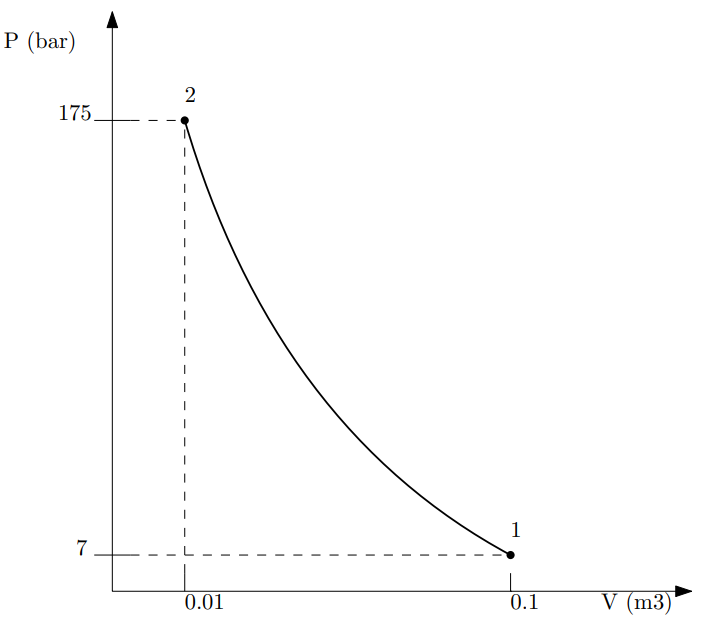
\includegraphics[width=0.5\linewidth]{F1.png}

		
		\question[12] 1kg of water at atmospheric pressure is heated in a constant pressure process from $25^oC$ to $250^oC$. Subsequently, the water is cooled in a constant volume process to saturated steam.
		\begin{itemize}
			\item Estimate the Temperature of the final state
			\item Draw the process on a P-v and T-v diagram
		\end{itemize}

		\textbf{Solution: }

		Water is in superheated state at $250^oC$ and 1 bar. The specific volume at state 2 is $2.4m^3/kg$ using Table A-4. More exactly, using interpolation:
	$$v_2=2.359+(2.546-2.359)\times\frac{1}{4}\ m^3/kg$$
	Note that process $2\to3$ is a constant volume process, so $v_2=v_3$. So we have to find (or estimate) a temperature in table A-3 or A-2, such that the specific volume of saturated vapor, $v_g$ is equal to $v_3$. The closest match is at $P=0.7\ bar$ and $T=89.95^oC$, with $v_g=2.365$.
	So $T_3\approx89^oC$. More precisely, $T_3=89.48^oC$
		
		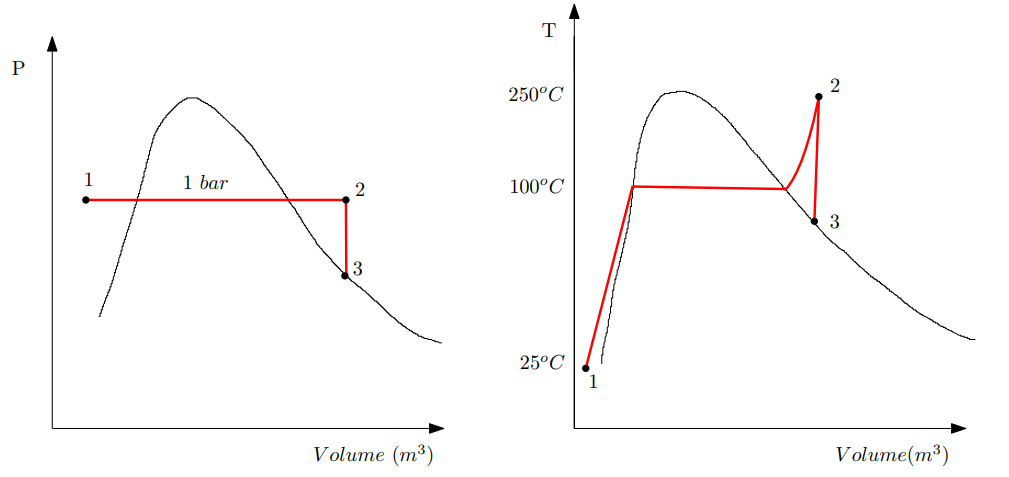
\includegraphics[width=\linewidth]{F2.png}
		
		\question[6] Determine the heat transfer rate per unit area for a 25 cm thick concrete wall with a temperature of $10^o$C on one end and a temperature of $26^o$C on the opposite end. The thermal conductivity for concrete is 0.7 W/(m K)

		\textbf{Solution: }

		$$\frac{\dot{Q_x}}{A}=-k\frac{dT}{dx}=-0.7\times \frac{26-10}{0.25}=-44.8\ W/m^2$$
		\question[6] Find the quality of a saturated liquid-vapor mixture of water at $T=100^\circ\text{C}$ and $u=1800 kJ/kg$

		\textbf{Solution: }

		The specific internal energy is given by:
		$$u=u_f+xu_{fg}$$
		$$\to x=\frac{u-u_f}{u_g-u_f}=\frac{1800-418.94}{2506.5-418.94}=0.661$$
		\question[4] Find the Volume of 7.6 kg of Saturated Steam at 900 kPa pressure

			\textbf{Solution: }

			Using Table A-3, at 9 bar: $v=0.2150 m^3/kg$
			So Volume $V=7.6\times0.2150=1.634\ m^3$
		\question[3] A mercury barometer is used to measure atmospheric pressure. Estimate the height of the mercury column in inches, given the specific weight of mercury $\lambda=\rho g=0.49\ lb/in^3=133.7\ kN/m^3$ and $1\ atm=14.7\ psi=101.325\ kPa$

		\textbf{Solution: }

		$$\rho gH=14.7\ psi\to H=14.7/0.49 = 30\ inch$$
		
			\question[3] Find the Enthalpy of Vaporization (Latent heat of vaporization) of water at 10 bar

				\textbf{Solution: }

				Using Table A-3 at 10 bar, Enthalpy of Vaporization:
				$$h_{fg}=2015.3\ kJ/kg$$
				
		\question[12] In an automobile, the tires are pressurized with the gage pressure set at 30 pounds per square inch gage (psig) when the temperature of air is $30^\circ\text{C}$. The temperature drops to $8^\circ\text{C}$. What will be the gage pressure in the tires?
		
		\question[10] Air in a piston-cylinder assembly undergoes isothermal expansion. i.e. A polytropic process ($Pv^n=$ constant) with n=1. \\
		The initial state of the Air is $P_1=7\ bar ;\quad V_1=0.1 m^3$ 
		\begin{itemize}
			\item Compute the work done if the air expands to $V_2=0.5\ m^3$
			\item Determine the heat transfer during the process
			\item Draw the process on a P-v diagram
		\end{itemize}

		
		\question[18] 2 kg of water undergoes the following processes:
		\begin{itemize}
			\item \textbf{Process 1 to 2:} Constant Pressure Heating at 10 bar from $80^\circ\text{C}$ to saturated vapor state.
			\item \textbf{Process 2 to 3:} Constant volume cooling with a heat transfer of -300 kJ. (Heat removed from the system)
		\end{itemize}
		
		
		Determine the Specific Volume (v), Specific Internal Energy (u), and Quality (x) at the final state. Draw the processes on a T-v and P-v diagram
		
		\question[10] Compute the work done in expansion of water initially in the mixed region with $x=0.4$ to saturated vapor at a constant pressure of 6 bar.
		
		\question[10] In an automobile, the tires are pressurized with the gauge pressure set at 30 pounds per square inch gauge (psig) when the temperature of air is $30^\circ\text{C}$. The temperature drops to $8^\circ\text{C}$.
			\begin{enumerate}
				\item[(a)] Estimate the gauge pressure in the tires in psig?
				\item[(b)] If the volume of the tire is 10 liters, estimate the mass of air that must be added to the tire to bring the pressure in the tire back to 30 psig ($1\text{ liter} = 1000\text{ cm}^3$)
			\end{enumerate}
		\question[10] One kg of water vapor is heated in a closed tank at constant pressure from saturated vapor at $180^\circ\text{C}$ to a final temperature of $350^\circ\text{C}$. Determine the initial and final volume and sketch the process on $T\text{--}v$ and $p\text{--}v$ diagrams.
		\question[10] Ammonia enters a control volume operating at steady state at $p_1 = 14 \text{ bar}$, $T_1 = 28^\circ\text{C}$, with a mass flow rate of $0.5 \text{ kg/s}$. Saturated vapor at $4 \text{ bar}$ leaves through one exit, with a volumetric flow rate of $1.036 \text{ m}^3\text{/min}$, and saturated liquid at $4 \text{ bar}$ leaves through a second exit. Determine
			\begin{enumerate}
				\item[(a)] the minimum diameter of the inlet pipe, in cm, so the ammonia velocity does not exceed $20 \text{ m/s}$.
				\item[(b)] the volumetric flow rate of the second exit stream, in $\text{m}^3\text{/min}$.
			\end{enumerate}
		\question[18] Air in a piston-cylinder assembly initially has a volume of 50 $cm^3$ at $T_1=760 K$ and  $P_1=2400$ kPa. The specific heat at constant pressure, may be assumed to have a constant value of $c_p=1.108$ kJ/kg K
			\begin{itemize}
				\item Process $1\to 2$: The air undergoes a constant volume heat addition to $T_2=1500 K$. Compute the mass of the air, the heat added (in kJ) and the Pressure $P_2$ (in kPa)
				\item Process $2\to 3$: The air undergoes a constant pressure heat addition of 0.167 kJ. Compute the final pressure $P_3$ and volume $V_3$  
				\item Draw the process on a P-v diagram
			\end{itemize}
			

			\textbf{Solution: }

			Process $1\to 2$:

			$$m=\frac{PV}{RT}=\frac{2400\times 50\times 10^{-6}}{0.287\times760}=5.5\times 10^{-4} kg$$
			$$Q_{12}=m(u_2-u_1)=mc_v(T_2-T_1)=0.3342\ kJ$$
			$$\frac{P_2}{P_1}=\frac{T_2}{T_1}\to P_2=\frac{P_1T_2}{T_1}=4737\ kPa$$

			Process $2\to 3$:

			$$Q_{23}=m(h_3-h_2)=mc_p(T_3-T_2)$$
			$$\to T_3=T_2+\frac{Q_{23}}{mc_p}=1774\ K$$
			$$P_3=P_2=4737\ kPa$$
			$$\frac{V_3}{V_2}=\frac{T_3}{T_2}\to V_3=59.14\ cm^3$$

			\question[12] 
		Complete the below table, for Water (Values in Red are the answers):
		\begin{center}
			
			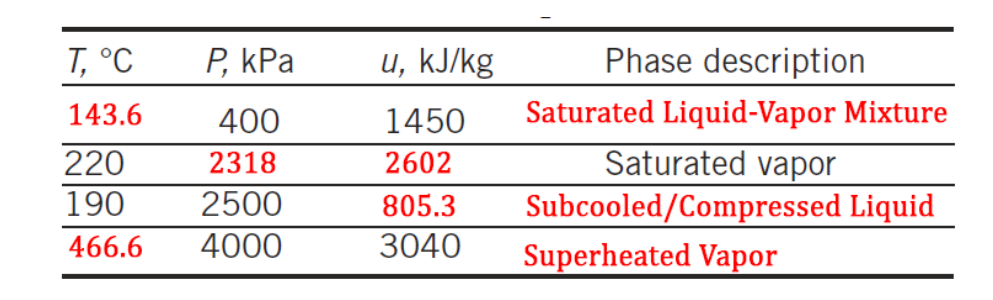
\includegraphics[width=0.6\linewidth]{table.png} \\
			
		\end{center}
		
		\question[18] Steam enters an insulated Turbine at $T=360^o\ C$ and $P=3$ MPa with a mass flow rate of 9.2 kg/s. 20\% of the entering mass flow exits the turbine at 0.5 MPa and $180^o\ C$. The rest exits the Turbine from another location at 10 kPa and a quality of 90\%. If the Inlet Velocity is 26.5 m/s, estimate the inlet piping diameter.
			\\
			\textbf{Solution: } 
			\\
			$$\dot{m}=\frac{A_1\overrightarrow{V_1}}{v_1}=\frac{\pi d^2}{4v_1}\overrightarrow{V_1}=9.2\ kg/s $$
			Specific Volume at the inlet, from superheated table @ 3 MPa, $360^o$C:
			$$v_1=0.0923\ m^3/kg$$
			$$\to d=0.202\ m$$
			
			Mass flow rate at the first and second exit:
			$$\dot{m_2}=0.2\dot{m_i}=1.84\ kg/s$$
			$$\dot{m_3}=0.8\dot{m_i}=7.36\ kg/s$$
			

	\end{questions}
\end{document}
